\section{C.~~Mode mixing due to nonlinearities}
\makeatletter
\protected@edef\@currentlabel{C}
\label{sec:mode mixing}
\makeatother
\renewcommand\thefigure{\thesection C.\arabic{figure}} %To set the Fig numbering to B
\setcounter{figure}{0} 

The signal detected by the SQUID contains not only the six modes related to the six degrees of motion of the magnetic particle (three librations and three translations). It also contains other vibrational movement of the setup. Modes of the mass spring system are most prominent in the \SIrange{0.5}{15}{Hz} range, see Fig.~\ref{fig:spectrum_mass_spring}. 

\begin{figure}[h]
    \centering
    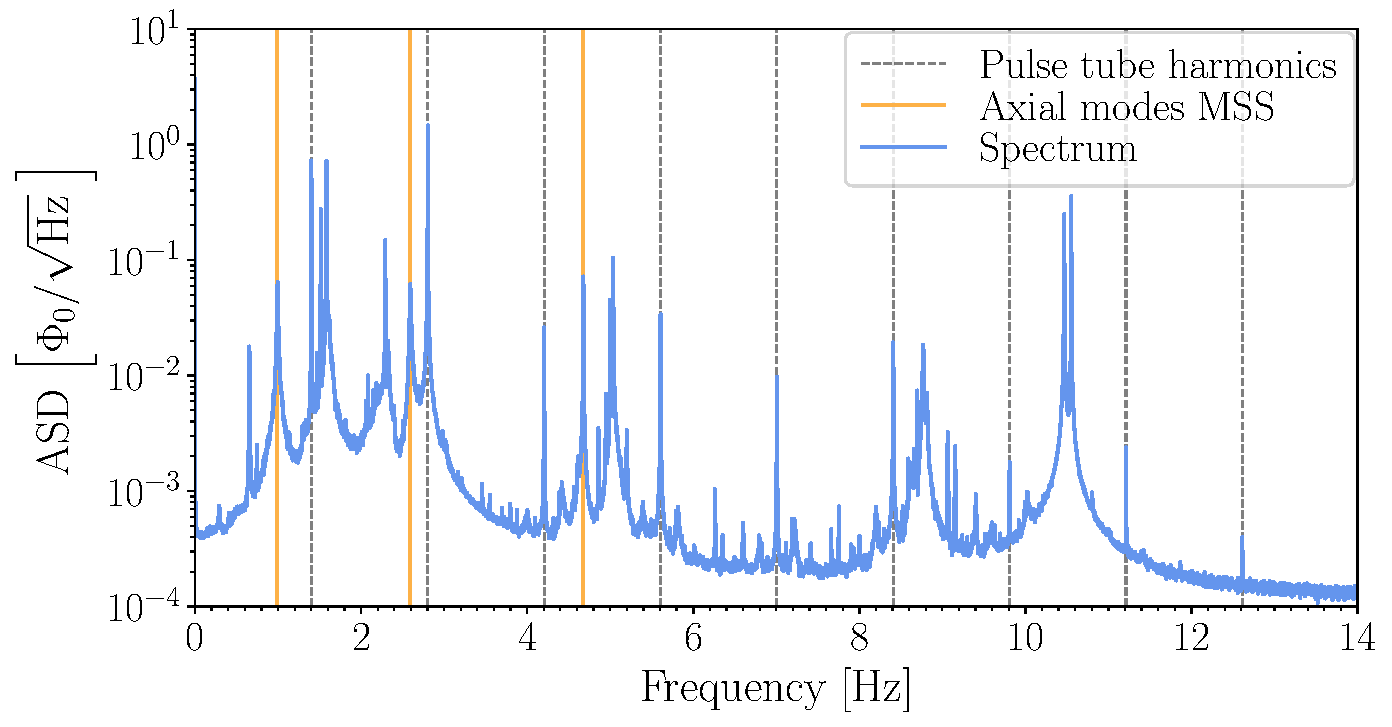
\includegraphics[width=\columnwidth]{5-Appendix/Figures/paper_spectrum_mass_spring_small_good2.pdf}
    \caption{Typical ASD of the resonances of the mass spring system as measured by the SQUID that measures the relative motion between the levitated magnet and pick-up coil. Multiples of the pulse tube frequency (\SI{1.401}{Hz}) are indicated with the vertical dashed lines. The axial modes of the mass spring system (MSS) as simulated are indicated with the vertical lines.}
    \label{fig:spectrum_mass_spring} 
\end{figure}

Many of these peaks in the spectrum can be attributed to vibrations caused by either the cooling equipment or the resonances of the vibration isolation system. Using a finite element model, we can link certain frequencies to modes of the mass spring system (MSS).

In Fig.~\ref{fig:spectrum_attenuation}, a finite element simulation transfer function is plotted of both the lateral and axial motion of the MSS to the experiment. To generate these plots, a simplified model is solved using a finite element method. Here, the three masses are simulated as perfect cylinders, and the helical springs are idealized as perfectly elastic snare springs, and their spring constants are physically measured at room temperature and extrapolated to cryogenic temperatures.

We observe that the simulated axial modes (vertical motion) of the MSS align directly with some of the measured peaks in the spectrum. Other peaks in the spectrum can be explained by the lateral and rotational movement of the mass spring system. Comparing between the simulation and the measurements, the values do not all coincide, but some are shifted with the highest mode at \SI{10.5}{Hz}.

\begin{figure}[h]
    \centering
    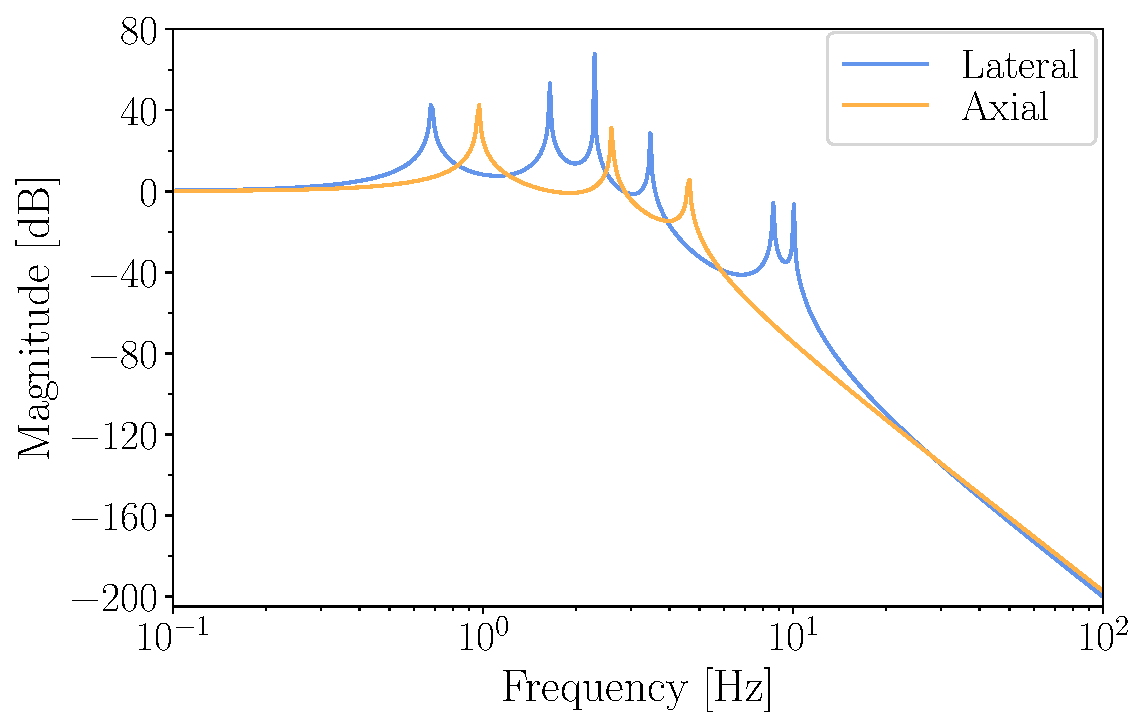
\includegraphics[width=\columnwidth]{5-Appendix/Figures/paper_spectrum_attenuation_log10.pdf}
    \caption{Bode magnitude plot of the attenuation of both the lateral and axial motion of the mass spring system (MSS), simulated with a finite element model.}
    \label{fig:spectrum_attenuation}
\end{figure}

During the experiment, we also observe peaks in the spectrum at frequencies that are the sum or difference of two peaks elsewhere in the spectrum. The most clear example can be seen in Fig.~\ref{fig:upconversion_mode_3} at \SI{51.5}{Hz}, where the peak displaced by \SI{0.92}{Hz} to the left of the resonance at a frequency of \SI{49.67}{Hz} is clearly reflected in the resonance of the magnet to \SI{51.51}{Hz}. This upconverted noise is cooled simultaneously with the resonance peak, meaning that the noise is coupled in through the motion of the magnet, the amplitude of the mode decreases with increasing gain and also the \SI{51.5}{Hz} noise decreases with increasing gain. We attribute the noise peak at \SI{49.67}{Hz} to a snare mode of the bottom spring of the vibration isolation system that we find in some finite element simulations. This mixing occurs because of the non-linearity of the trapping potential, which arises from the non-linear magnetic potential.

\begin{figure}[h]
    \centering
    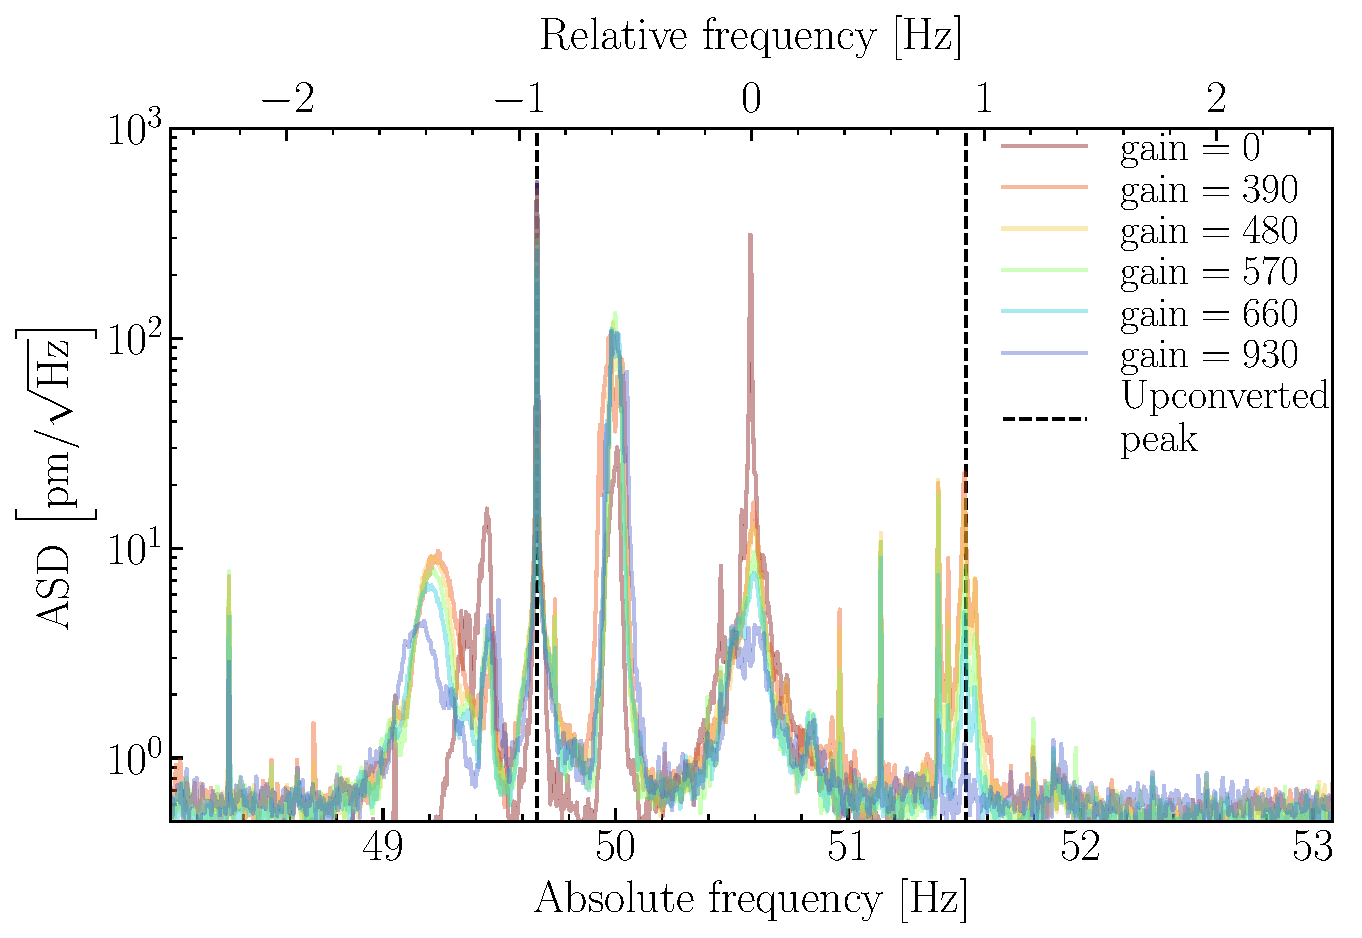
\includegraphics[width=\columnwidth]{5-Appendix/Figures/paper_appendix_upconversion_mode_3.pdf}
    \caption{The spectrum around mode 3, where upconversion can be seen at for example \SI{51.5}{Hz}.}
    \label{fig:upconversion_mode_3} 
\end{figure}

Please note that when we perform mode cooling and bring the particle motion of a translational mode down to a few picometers, the amplitude of the relative motion between the magnet and the trap at lower frequencies (\SIrange{0.5}{15}{Hz}) remains unchanged, and can be more than four orders of magnitude in amplitude larger as is visible in Fig~\ref{fig:spectrum}. For the \SI{50.6}{Hz} mode, mechanical vibrations of the compressor and circulation pumps of the dilution refrigerator (which are often slightly below \SI{50}{Hz}) mix with the mechanical modes of the vibration isolation system. We cannot account for all the peaks we see, but we attribute this to upconversion of several peaks mixing together to work against us. Also we cannot exclude that \SI{50}{Hz} electrical noise interferes with mechanical vibrations. Therefore we conclude that to improve the feedback cooling further we will need to also perform linear feedback cooling on the modes of the vibration isolation system.




%In Fig.~\ref{fig:upconversion_mode_3} and Fig.~\ref{fig:upconversion_mode_4} we show the upconversion around the two cooled modes. The most clear example can be seen in Fig.~\ref{fig:upconversion_mode_3} at \SI{51.5}{Hz}, this upconverted noise is cooled simultaneously with the resonance peak. Meaning that the noise is coupled in through the motion of the magnet, the amplitude of the mode decreases with increasing gain and also the \SI{51.5}{Hz} noise decreases with increasing gain.

